\documentclass[11pt]{article}

\usepackage[utf8]{inputenc}
\usepackage[T1]{fontenc}
\usepackage{lmodern}
\usepackage{microtype}
\usepackage{amsmath,amsfonts}
\usepackage{graphicx}
\usepackage{booktabs}
\usepackage{hyperref}
\usepackage{enumitem}
\usepackage{geometry}
\usepackage{parskip}

\geometry{margin=1in}

\title{\textbf{EvaluatorDPT: Auditable Bounded Decision Control with Learned Deferral}}

\author{
Sankaranarayanan Palamadai Chandrasekaran \\
Simple Machine Mind \\
\texttt{sankar@smsquared.ai}
}

\date{}

\begin{document}

\maketitle

\begin{abstract}
Production AI systems frequently operate under incomplete, conflicting, or insufficient evidence. Forced classifiers collapse such cases into action labels, while free-form generative systems can produce outputs that are difficult to audit as execution decisions. This paper presents EvaluatorDPT, a bounded decision-control model that predicts YES, NO, or TBD, where TBD is learned as a first-class deferral outcome rather than applied only as a post-hoc confidence rule. The model uses a transformer encoder with a primary bounded-decision head and structured auxiliary channels for values and emotions/sentiments. For the current S12B publish candidate, we report decision performance on DS-L validation and test splits, with auxiliary emotion metrics intentionally omitted because the emotion head is masked in this lineage. On the full DS-L test split (n=44,597), S12B achieves Accuracy = 0.8260 and Macro F1 = 0.8252, with per-class F1 of 0.8314 (YES), 0.8486 (NO), and 0.7956 (TBD). Beyond top-line metrics, the release includes calibration evidence (ECE = 0.0338 on validation), threshold-sweep artifacts, multi-seed stability checks, confusion matrices, reproducibility commands, and a certifier-facing evidence bundle. The central contribution is an auditable decision interface: learned deferral, bounded outputs, confidence-aware thresholding, and packaged certification artifacts for governed AI routing under ambiguity.
\end{abstract}

\section{Introduction}

AI systems increasingly sit between language inputs and downstream actions. In such settings, the operational question is not only whether a model can classify text, but whether it can provide a governed decision interface: act, block, or defer. Inputs may be incomplete, contradictory, or ambiguous; forcing a YES or NO decision in these cases produces brittle automation and weak auditability.

EvaluatorDPT addresses this problem by modeling decision control as a bounded three-way output space:
\[
\mathcal{Y}_d = \{\text{YES}, \text{NO}, \text{TBD}\}.
\]
The TBD outcome is not merely a post-hoc rejection threshold. It is a learned class that allows the model to internalize deferral boundaries during training. Thresholding remains useful at deployment time, but it is applied on top of a model that already represents ambiguity as part of the label space.

The signature contribution of this work is \textbf{learned deferral as an auditable decision-control interface}. The model does not generate free-form decisions. It emits bounded labels, confidence scores, and structured auxiliary signals, and the release packages the evidence needed to inspect and certify the behavior: calibration, threshold sweeps, multi-seed stability, confusion matrices, and reproducibility artifacts.

\paragraph{Contributions.}
\begin{itemize}[leftmargin=1.5em]
  \item We formulate decision routing as bounded control over YES, NO, and learned TBD deferral.
  \item We present a transformer-based multi-head architecture that separates primary decision prediction from structured auxiliary context signals.
  \item We evaluate the S12B publish candidate on full validation and test splits and report per-class behavior, calibration, threshold-sweep evidence, and stability checks.
  \item We provide a certifier-facing artifact structure that turns model evaluation into a reviewable evidence bundle rather than a single headline score.
\end{itemize}

\section{Related Work}

EvaluatorDPT is related to selective classification and reject-option models, which abstain from prediction under uncertainty \cite{elyaniv2010selective, geifman2017selective, franc2023reject}. In many such systems, abstention is applied after prediction using confidence thresholds. EvaluatorDPT differs by learning a deferral label directly while still preserving threshold sweeps for operating-point selection.

The architecture builds on transformer language models such as BERT \cite{devlin2019bert} and multi-task learning \cite{caruana1997multitask}. The distinction in this work is operational: auxiliary outputs are treated as structured context signals available at inference time rather than only as training regularizers.

Calibration is also central. Neural confidence scores can be miscalibrated \cite{guo2017calibration}, so EvaluatorDPT pairs decision outputs with calibration evidence and threshold-sweep artifacts. This is relevant for governance because the operating policy should be inspectable rather than implicit.

\section{System Overview}

The model receives a context signal and returns:
\begin{itemize}[leftmargin=1.5em]
  \item a bounded decision: YES, NO, or TBD;
  \item decision confidence derived from the primary decision head;
  \item structured auxiliary signals for values and emotions/sentiments, where enabled by the lineage;
  \item evidence artifacts that support threshold selection and audit.
\end{itemize}

\begin{figure}[h]
\centering
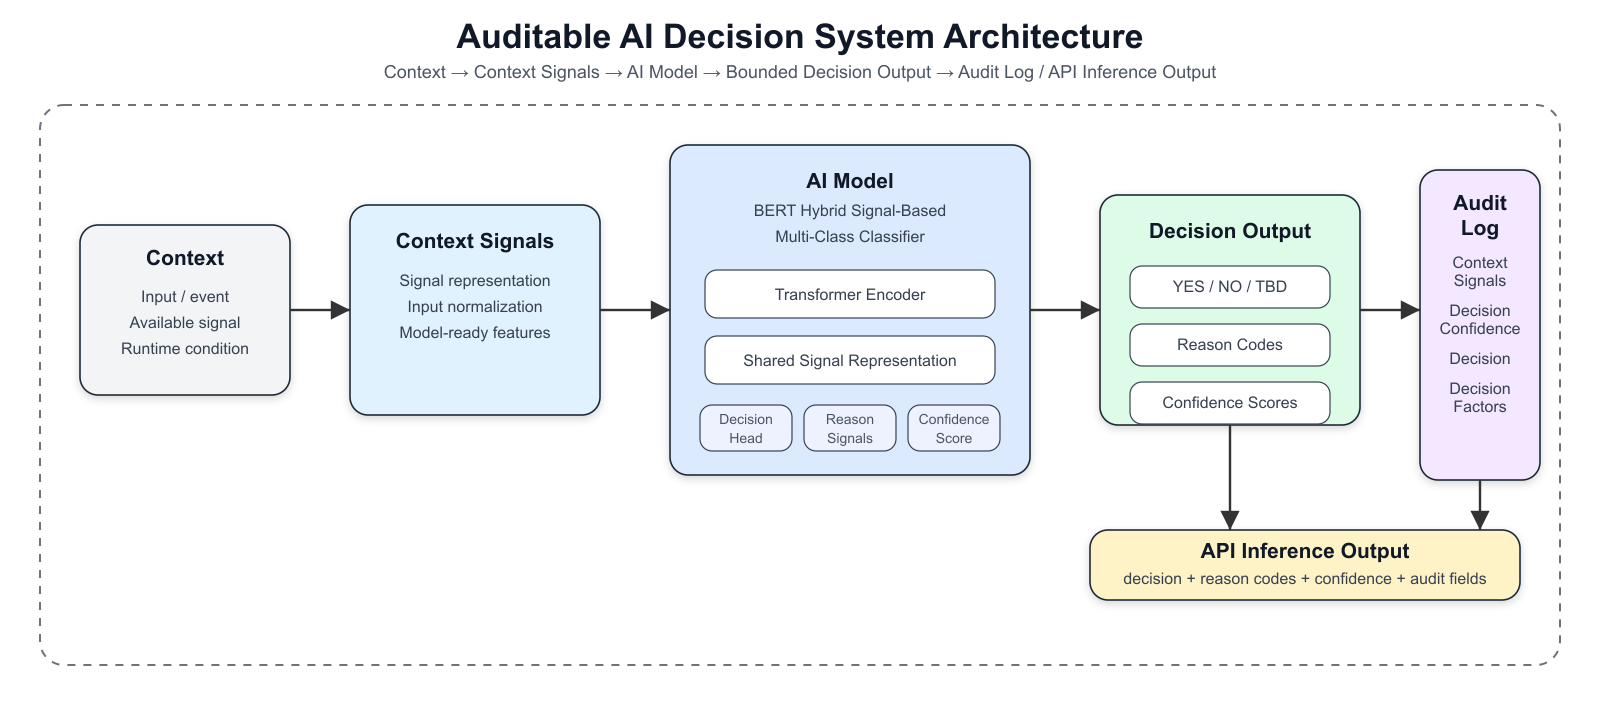
\includegraphics[width=0.9\linewidth]{architecture.png}
\caption{EvaluatorDPT system architecture: tokenized decision event to shared transformer encoder, bounded decision output, confidence, and structured auxiliary channels.}
\end{figure}

\section{Methodology}

\subsection{Bounded Decision Formulation}

Let $x$ be a decision-event input. EvaluatorDPT predicts a primary decision distribution over $\mathcal{Y}_d = \{\text{YES}, \text{NO}, \text{TBD}\}$. The TBD label represents explicit deferral under insufficient semantic certainty. This differs from binary classification followed by confidence filtering because the model learns examples of deferral as part of the supervised task.

Deployment policies may still choose operating thresholds over the predicted probabilities. In this formulation, thresholding is an operating policy layered over a bounded decision model, not the sole mechanism by which uncertainty is represented.

\subsection{Architecture}

EvaluatorDPT uses a BERT-base encoder \cite{devlin2019bert} with a maximum sequence length of 128 tokens. The shared encoder feeds task-specific heads:
\begin{itemize}[leftmargin=1.5em]
  \item a primary three-class decision head;
  \item a 10-label value head;
  \item a 28-label emotion/sentiment head.
\end{itemize}

For S12B, the decision head is the validated output reported in this paper. The emotion head is masked in the DS-L lineage, so emotion metrics are intentionally not claimed for this release candidate. The auxiliary-head architecture remains part of the interface design, but this paper scopes empirical claims to the validated S12B decision behavior and certification evidence.

\subsection{Boundary Refinement}

A recurring challenge in bounded decision systems is the boundary between action and deferral. S12B uses DS-L with a targeted boundary pack that focuses on hard semantic regions such as contradiction, negation, low lexical overlap entailment, high lexical overlap contradiction, long-text stress cases, and hedge/modal ambiguity. This is a controlled refinement strategy: the goal is to improve boundary behavior using targeted examples rather than relying only on broad dataset scale.

\section{Evaluation Setup}

The current publish candidate is \texttt{exp\_t90\_S12B\_boundarypack\_ep1\_fromS12ep3}. Results are reported for DS-L validation and test splits:
\begin{itemize}[leftmargin=1.5em]
  \item validation: n = 44,404;
  \item test: n = 44,597.
\end{itemize}

The release artifacts include full-split metrics, confusion matrices, calibration data, threshold sweeps, and reproducibility commands under the public certification bundle.

\section{Results}

\subsection{Decision Performance}

\begin{center}
\begin{tabular}{lcc}
\toprule
Split & Accuracy & Macro F1 \\
\midrule
Validation (n=44,404) & 0.8224 & 0.8213 \\
Test (n=44,597) & 0.8260 & 0.8252 \\
\bottomrule
\end{tabular}
\end{center}

\subsection{Per-Class Test Performance}

\begin{center}
\begin{tabular}{lrrrr}
\toprule
Class & Precision & Recall & F1 & Support \\
\midrule
YES & 0.8205 & 0.8425 & 0.8314 & 14,883 \\
NO & 0.8598 & 0.8376 & 0.8486 & 15,650 \\
TBD & 0.7955 & 0.7958 & 0.7956 & 14,064 \\
\bottomrule
\end{tabular}
\end{center}

\subsection{Validation Confusion Matrix}

\begin{center}
\begin{tabular}{lccc}
\toprule
 & Pred YES & Pred NO & Pred TBD \\
\midrule
True YES & 12,496 & 999 & 1,467 \\
True NO & 1,035 & 13,066 & 1,433 \\
True TBD & 1,793 & 1,160 & 10,955 \\
\bottomrule
\end{tabular}
\end{center}

\section{Audit and Certification Evidence}

EvaluatorDPT is packaged with audit artifacts in addition to evaluation scores. For S12B, the public certification pack is located at:
\begin{quote}
\texttt{certification/runs/S12B\_20260526/}
\end{quote}

The pack includes:
\begin{itemize}[leftmargin=1.5em]
  \item evaluation and calibration reports;
  \item calibration data with validation ECE = 0.0338;
  \item threshold-sweep artifacts for TBD-fallback operating policies;
  \item multi-seed stability evidence, with validation seeds 42, 0, and 7 producing identical Macro F1 (std = 0.0);
  \item run metrics, confusion matrix, diagnostics, and reproducibility commands.
\end{itemize}

This certification structure is part of the system contribution. It makes the model reviewable by exposing the evidence needed to inspect operating behavior, not just the final checkpoint.

\section{Discussion}

The results show that bounded decision control can be evaluated as a decision interface rather than as ordinary classification alone. S12B achieves balanced performance across YES, NO, and TBD, with NO F1 = 0.8486 and TBD F1 = 0.7956 on the full test split. The remaining difficulty is the boundary between actionable decisions and deferral, especially ambiguous cases where a human or downstream policy may prefer conservative routing.

The audit evidence is as important as the score. Calibration, threshold sweeps, and multi-seed stability make the model's operating behavior inspectable. This supports the claim that the model is suitable as a governed routing layer: downstream systems can select operating thresholds and document tradeoffs without retraining the core model.

The auxiliary architecture also matters, but empirical claims should remain scoped. In S12B, decision behavior is validated; emotion metrics are not reported because the emotion head is masked. Future releases can separately validate auxiliary value and emotion behavior as independent outputs.

\section{Limitations}

Results are specific to DS-L, the S12B checkpoint, and the evaluation setup reported here. Additional domains require separate validation. Inputs are truncated to 128 tokens, so long-context use cases require chunking or preprocessing. The emotion head is masked in this lineage, so this paper does not claim validated emotion-head performance for S12B. The dataset composition includes public NLP sources and curated decision examples, but raw training data is not redistributed in this repository. Users should consult original dataset licenses before reusing source datasets.

\section{Conclusion}

This paper presented EvaluatorDPT, an auditable bounded decision-control model with learned deferral. Its primary contribution is not only a three-class classifier, but a deployable decision interface: YES, NO, or TBD, paired with confidence, threshold sweeps, calibration evidence, stability checks, and a certifier-facing artifact pack. On the full DS-L test split, S12B achieves Accuracy = 0.8260 and Macro F1 = 0.8252, with per-class F1 scores of 0.8314 (YES), 0.8486 (NO), and 0.7956 (TBD). These results support learned deferral and audit-ready release packaging as practical components for governed AI decision routing under ambiguity.

\bibliographystyle{plain}
\bibliography{references}

\end{document}
